\section{Ogólne zagadnienia brzegowe II rzędu}
\subsection{Warunki brzegowe typu Dirichletta}

Rozważając najbardziej ogólne zagadnienie brzegowe rzędu II z warunkami brzegowymi typu Dirichletta postaci:

\[
\begin{cases}
\vspace{0.1cm} 
\hspace{0,1cm} a(x) u'' + b(x)u' + c(x)u =f(x) \\
\vspace{0.1cm}
\hspace{0,1cm}u|_{x=a} = u_{a} \\
\hspace{0,1cm}u|_{x=b} = u_{b}
\end{cases}
\]
, gdzie:
$x\in[a,b]$
\\
\\
Okazuje się że stosowanie schematów na pochodną różnego rzędu o tej samej dokładności skutkuje tym, że cała metoda jest również rzędu II.

\subsection{Cel ćwiczenia}
Na laboratorium otrzymaliśmy następujące równania dla których mieliśmy stworzyć rozwiązujący je algorytm.

a)
\[
\begin{cases}
\vspace{0.1cm} 
\hspace{0,1cm} u'' - 4u =-4x \\
\vspace{0.1cm}
\hspace{0,1cm}u|_{x=0} = 0 \\
\hspace{0,1cm}u|_{x=1} = 2
\end{cases}
\]
, gdzie:
$x\in[0,1]$
\\
Rozwiązanie analityczne: $\widetilde{u}(x) = e^2(e^4-1)^{-1} (e^{2x} - e^{-2x}) + x$
\\
\\
b)
\[
\begin{cases}
\vspace{0.1cm} 
\hspace{0,1cm} u'' -u'- 2u =cos(x) \\
\vspace{0.1cm}
\hspace{0,1cm}u|_{x=0} = -\dfrac{3}{10} \\
\hspace{0,1cm}u|_{x=\dfrac{\pi}{2}} = -\dfrac{1}{10}
\end{cases}
\]
, gdzie:
$x\in[0, \dfrac{\pi}{2}]$
\\
Rozwiązanie analityczne: $\widetilde{u}(x) = -\dfrac{1}{10}(sin(x) + 3cos(x))$
\\
\\
c)
\[
\begin{cases}
\vspace{0.1cm} 
\hspace{0,1cm} -x^2u'' +2xu' +2u=-4x^2 \\
\vspace{0.1cm}
\hspace{0,1cm}u|_{x=0} = 0 \\
\hspace{0,1cm}u|_{x=1} = 0
\end{cases}
\]
, gdzie:
$x\in[0,1]$
\\
Rozwiązanie analityczne: $\widetilde{u}(x) = x^2 - x$

\vspace{0.3cm}
Ponadto zaprezentujemy wykres porównujący rozwiązanie numeryczne z rozwiązaniem analitycznym, a także wykres błędu $||E||_{\infty}$ w zależności od liczby obranych węzłów (n).
%\begin{samepage}
\newpage
\subsection{Algorytm}
%\textbf{Warunek brzegowy Dirichleta (I rodzaju)}
Poniżej przedstawiony został algorytm rozwiązania powyższych równań z przykładowymi danymi wejściowymi z podpunktu a).


\begin{samepage}
    \begin{Shaded}
\begin{Highlighting}[]
\FunctionTok{clear}\NormalTok{, }\FunctionTok{clc}\NormalTok{;}
\CommentTok{# Dane wejściowe}
\NormalTok{f = @(x) -}\FloatTok{4}\NormalTok{*x;}
\NormalTok{g = @(x) }\FunctionTok{exp}\NormalTok{(}\FloatTok{2}\NormalTok{) * (}\FunctionTok{exp}\NormalTok{(}\FloatTok{4}\NormalTok{) - }\FloatTok{1} \NormalTok{)^-}\FloatTok{1} \NormalTok{* (}\FunctionTok{exp}\NormalTok{(}\FloatTok{2}\NormalTok{*x) - }\FunctionTok{exp}\NormalTok{(-}\FloatTok{2}\NormalTok{*x)) + x;}
\NormalTok{a = }\FloatTok{0}\NormalTok{;}
\NormalTok{b = }\FloatTok{1}\NormalTok{;}
\NormalTok{ax = @(x) }\FloatTok{1}\NormalTok{;}
\NormalTok{bx = @(x) }\FloatTok{0}\NormalTok{;}
\NormalTok{cx = @(x) -}\FloatTok{4}\NormalTok{;}
\NormalTok{ua = }\FloatTok{0}\NormalTok{;}
\NormalTok{ub = }\FloatTok{2}\NormalTok{;}
\NormalTok{c = b-a;}
\NormalTok{n = }\FloatTok{10}\NormalTok{;}
\NormalTok{h = c/(n+}\FloatTok{1}\NormalTok{);}
\NormalTok{x = }\FunctionTok{linspace}\NormalTok{((a+h),(b-h),n);}
\CommentTok{# Obliczenia}
\NormalTok{a1 = (-}\FloatTok{2} \NormalTok{.* ax(x) + cx(x) .*h^}\FloatTok{2}\NormalTok{) .* }\FunctionTok{diag}\NormalTok{(}\FunctionTok{eye}\NormalTok{(n));}
\NormalTok{A1 = }\FunctionTok{diag}\NormalTok{(a1);}
\NormalTok{a2 = (ax(x(}\FloatTok{2}\NormalTok{:n)) -}\FloatTok{1}\NormalTok{/}\FloatTok{2} \NormalTok{.* bx(x(}\FloatTok{2}\NormalTok{:n)) .*h)' .* }\FunctionTok{diag}\NormalTok{(}\FunctionTok{eye}\NormalTok{(n-}\FloatTok{1}\NormalTok{));}
\NormalTok{A2 = }\FunctionTok{diag}\NormalTok{(a2, -}\FloatTok{1}\NormalTok{);}
\NormalTok{a3 = (ax(x(}\FloatTok{1}\NormalTok{:n-}\FloatTok{1}\NormalTok{)) +}\FloatTok{1}\NormalTok{/}\FloatTok{2} \NormalTok{.* bx(x(}\FloatTok{1}\NormalTok{:n-}\FloatTok{1}\NormalTok{)) .*h)' .* }\FunctionTok{diag}\NormalTok{(}\FunctionTok{eye}\NormalTok{(n-}\FloatTok{1}\NormalTok{));}
\NormalTok{A3 = }\FunctionTok{diag}\NormalTok{(a3, }\FloatTok{1}\NormalTok{);}
\NormalTok{A = A1  + A2 + A3;}
\NormalTok{F = (h^}\FloatTok{2} \NormalTok{* f(x));}
\NormalTok{F(}\FloatTok{1}\NormalTok{) = F(}\FloatTok{1}\NormalTok{) - ua * (ax(}\FloatTok{1}\NormalTok{) - }\FloatTok{1}\NormalTok{/}\FloatTok{2} \NormalTok{* bx(}\FloatTok{1}\NormalTok{)*h);}
\NormalTok{F(n) = F(n) - ub * (ax(n) + }\FloatTok{1}\NormalTok{/}\FloatTok{2} \NormalTok{* bx(n)*h);}
\NormalTok{U = linsolve(A,F');}
\NormalTok{U = [ua U' ub];}
\NormalTok{X = [a x b];}
\CommentTok{# Wykres}
\FunctionTok{plot}\NormalTok{(X, U, X, g(X), }\StringTok{'ro'}\NormalTok{);}
\CommentTok{# Błąd}
\NormalTok{E = }\FunctionTok{max}\NormalTok{(}\FunctionTok{abs}\NormalTok{(g(X) - U));}
\end{Highlighting}
\end{Shaded}


\end{samepage}

\newpage

\subsection{Wykresy}

a)\\
\begin{samepage}
Dla 10 węzłów:

\FloatBarrier
\begin{figure}[!ht]
    \begin{center}
        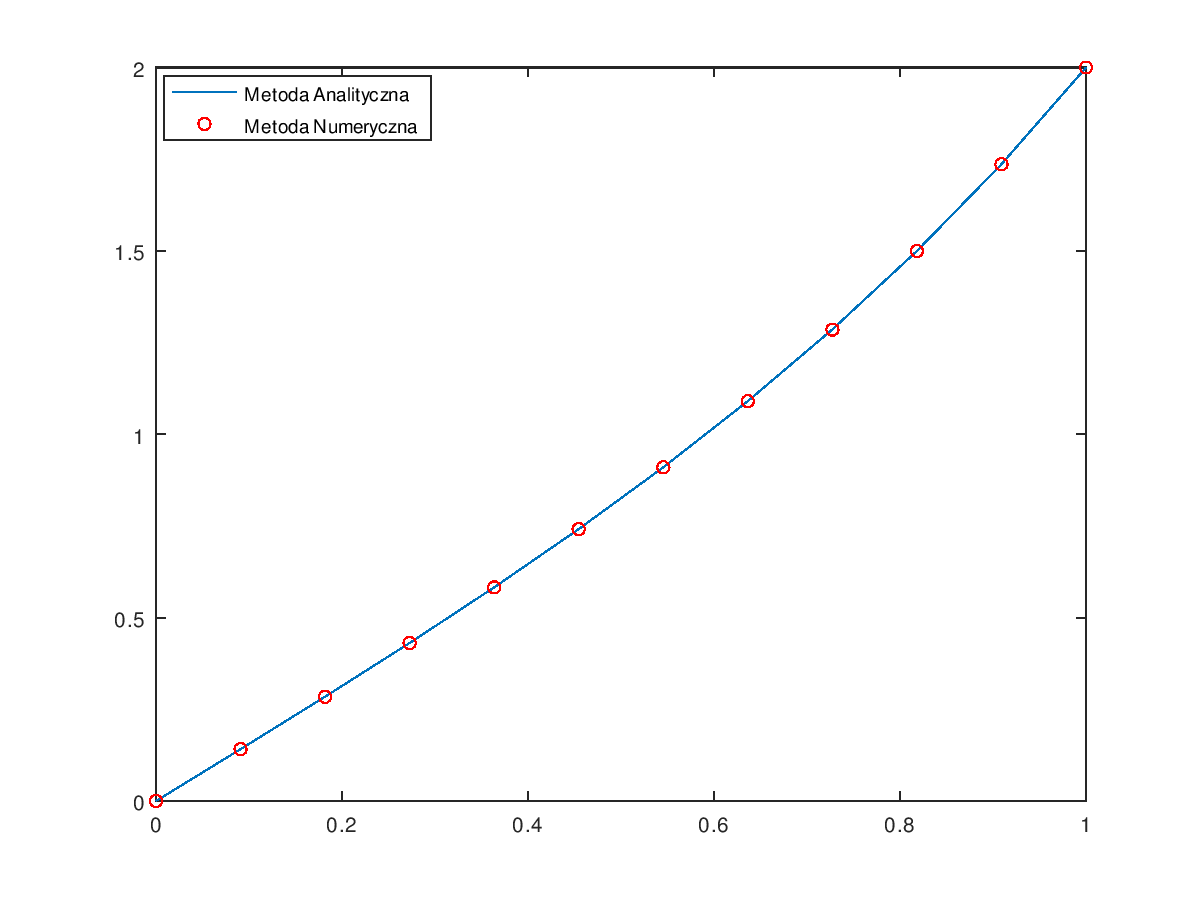
\includegraphics[width=0.8\textwidth]{Lab4/charts/zad1/zad1_n_10.png}
    \end{center}
    %\caption{Schemat logiczny w edytorze LAD oraz tabela symboli}
    %\label{fig:picture}
\end{figure}
\FloatBarrier
\end{samepage}

\begin{samepage}
Dla 25 węzłów:
\begin{figure}[!ht]
    \begin{center}
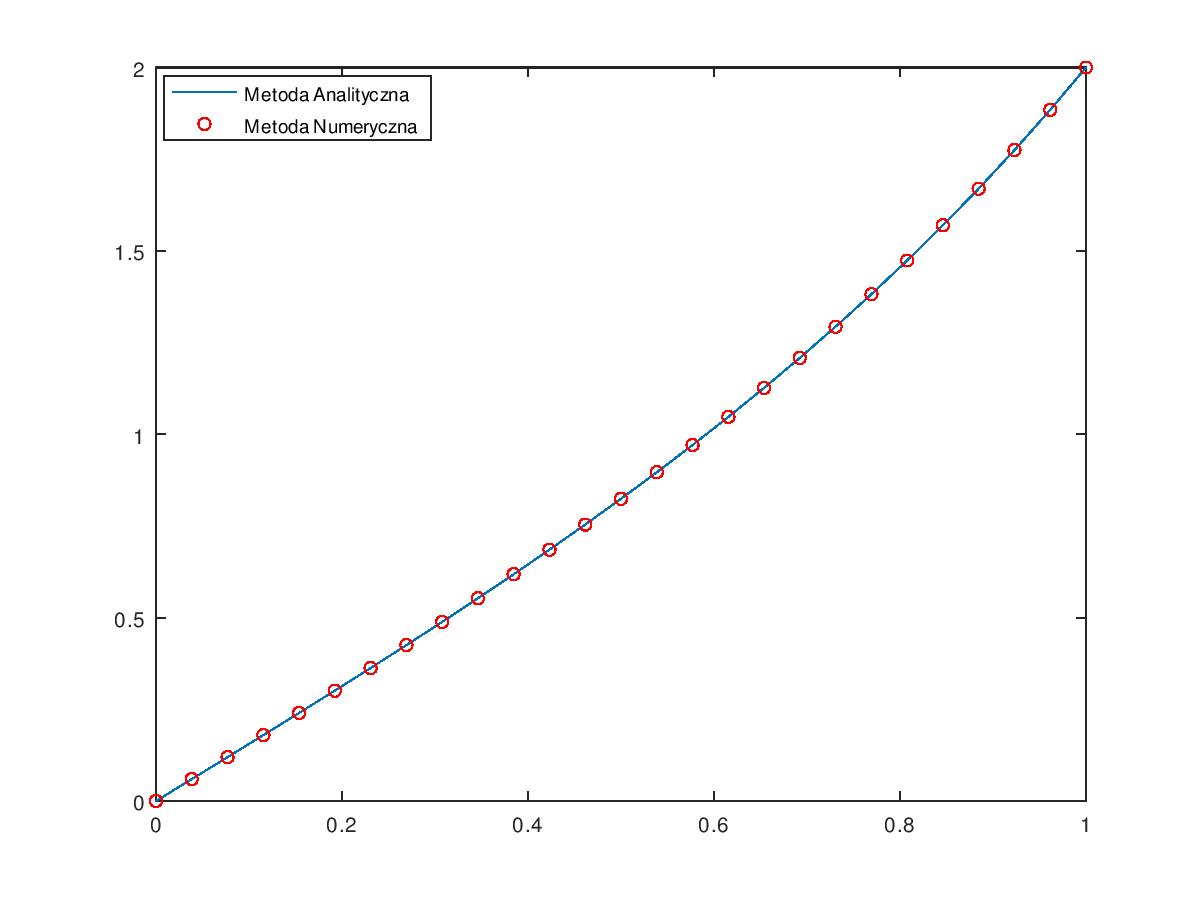
\includegraphics[width=0.8\textwidth]{Lab4/charts/zad1/zad1_n_25.png}
    \end{center}
    %\caption{Schemat logiczny w edytorze LAD oraz tabela symboli}
    %\label{fig:picture}
\end{figure}
\FloatBarrier
\end{samepage}

\newpage
\begin{samepage}
    
Dla 100 węzłów:
\begin{figure}[!ht]
    \begin{center}
    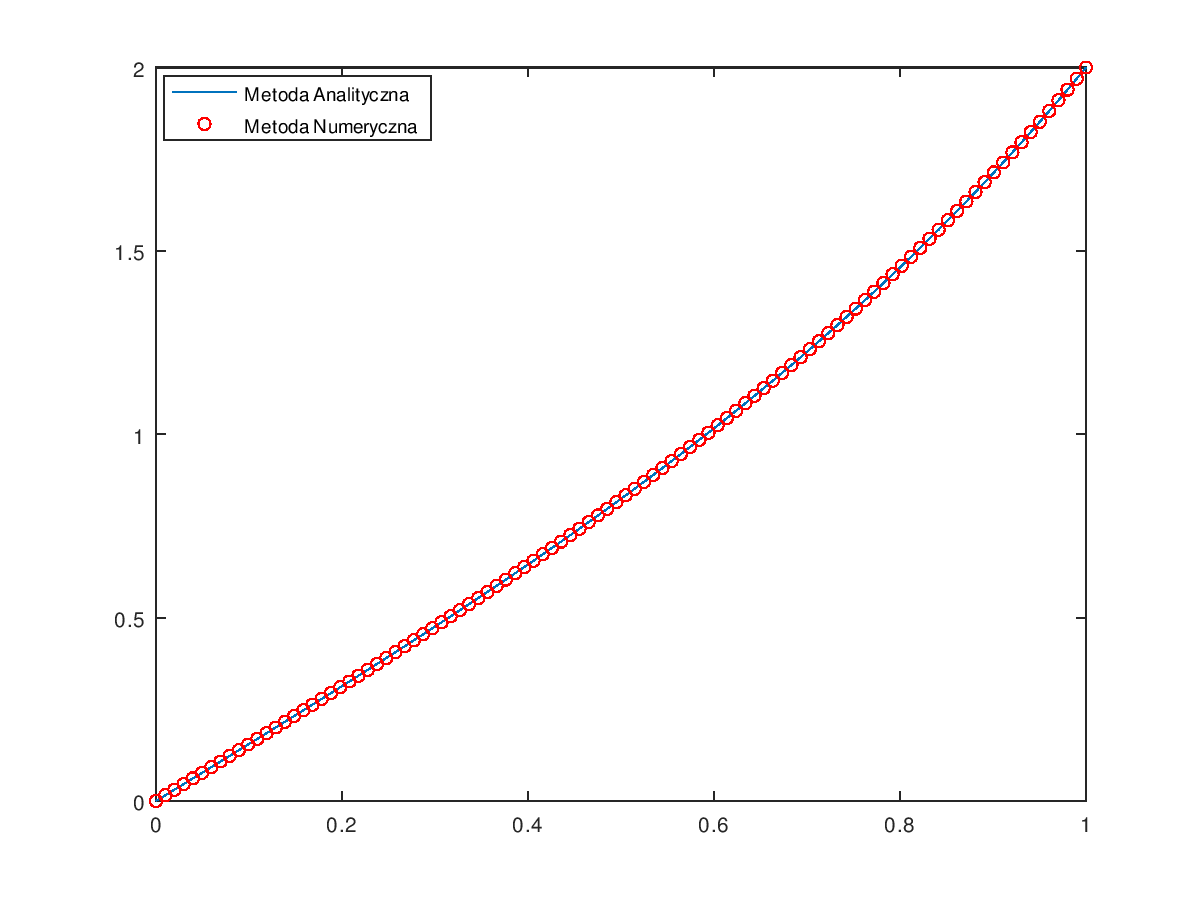
\includegraphics[width=0.8\textwidth]{Lab4/charts/zad1/zad1_n_100.png}
    \end{center}
    %\caption{Schemat logiczny w edytorze LAD oraz tabela symboli}
    %\label{fig:picture}
\end{figure}
\FloatBarrier
\end{samepage}
    
\begin{samepage}
Dla 1000 węzłów:

\begin{figure}[!ht]
    \begin{center}
    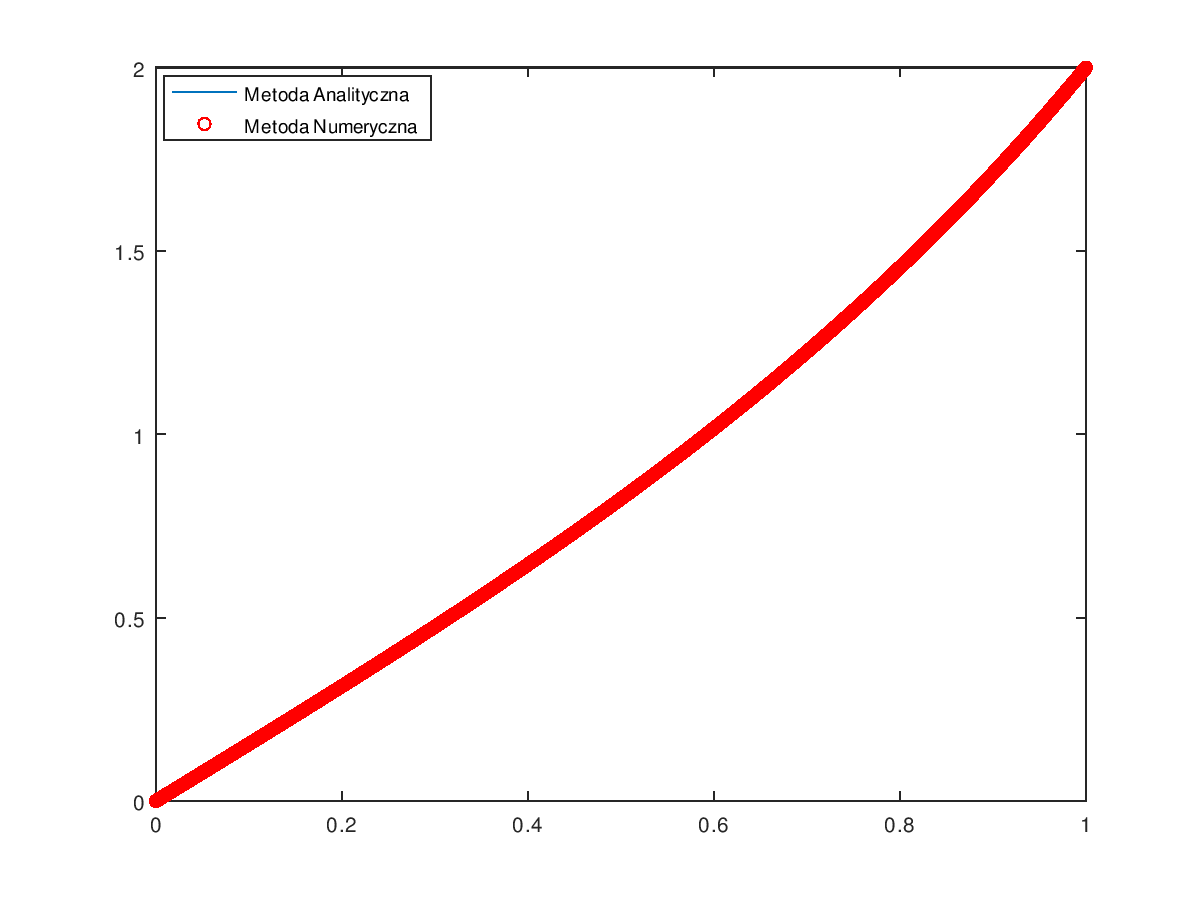
\includegraphics[width=0.8\textwidth]{Lab4/charts/zad1/zad1_n_1000.png}
    \end{center}
    %\caption{Schemat logiczny w edytorze LAD oraz tabela symboli}
    %\label{fig:picture}
\end{figure}
\FloatBarrier
\end{samepage}    

\newpage

\begin{samepage}
Błąd metody w zależności od liczby węzłów:
    \begin{figure}[!ht]
        \begin{center}
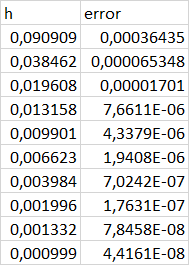
\includegraphics[width=0.8\textwidth]{Lab4/charts/zad1/error_dane.png}
        \end{center}
        %\caption{Schemat logiczny w edytorze LAD oraz tabela symboli}
        %\label{fig:picture}
    \end{figure}
    \FloatBarrier
\end{samepage} 

\begin{samepage}
    
    \begin{figure}[!ht]
        \begin{center}
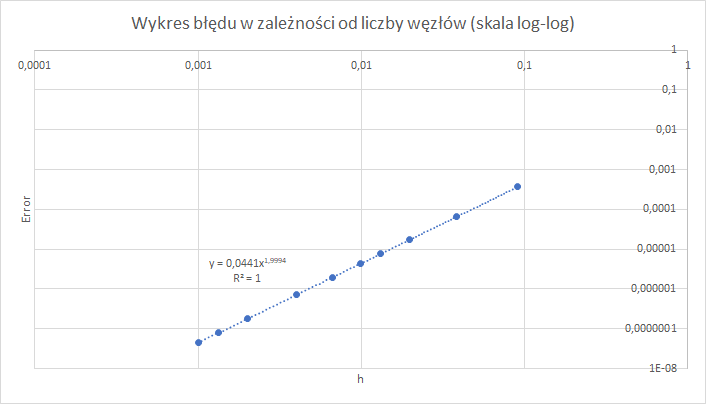
\includegraphics[width=0.8\textwidth]{Lab4/charts/zad1/error.png}
        \end{center}
        %\caption{Schemat logiczny w edytorze LAD oraz tabela symboli}
        %\label{fig:picture}
    \end{figure}
    \FloatBarrier
\end{samepage} 


\newpage
b)\\
\begin{samepage}
    Dla 10 węzłów:
    
    %{\centering
    
    %   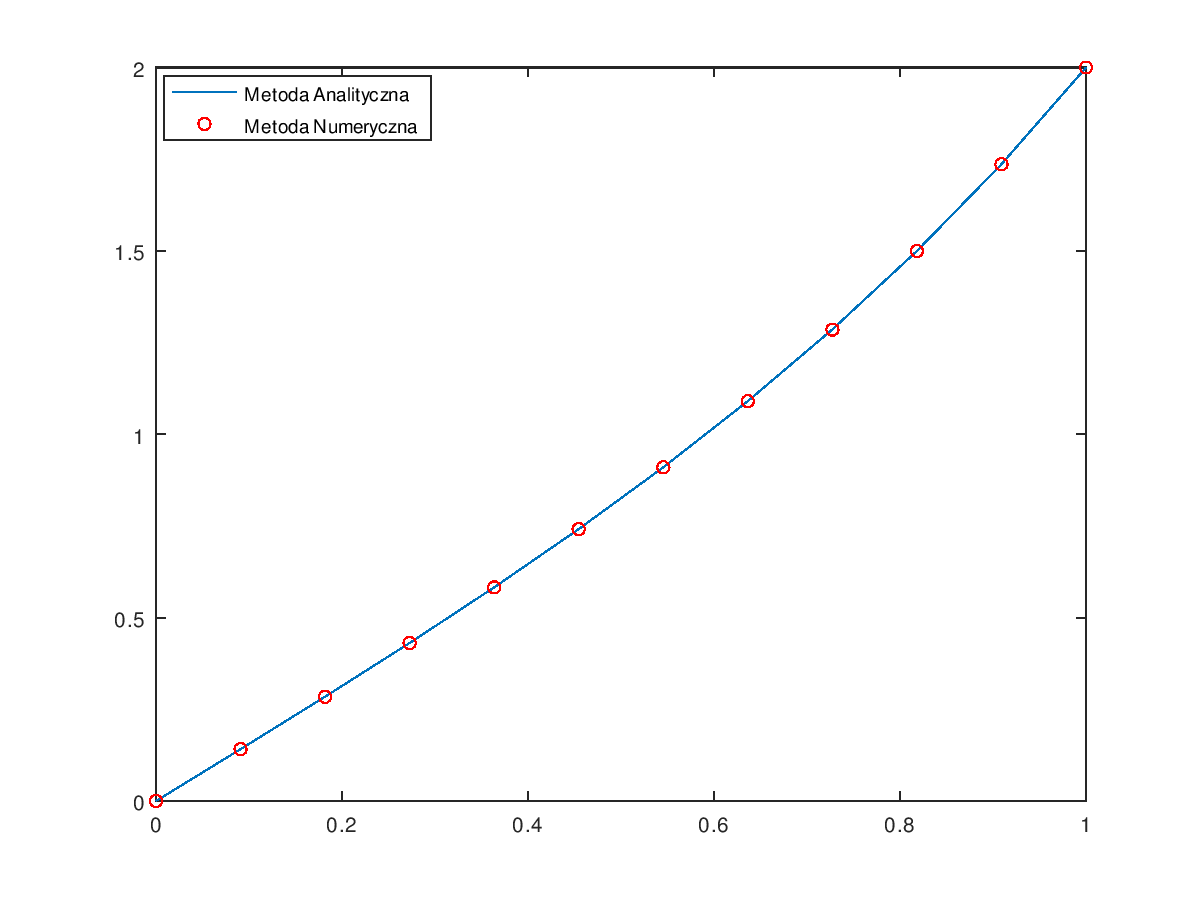
\includegraphics{Lab4/charts/zad1/zad1_n_10.png}
    
    %}
    \FloatBarrier
    \begin{figure}[!ht]
        \begin{center}
            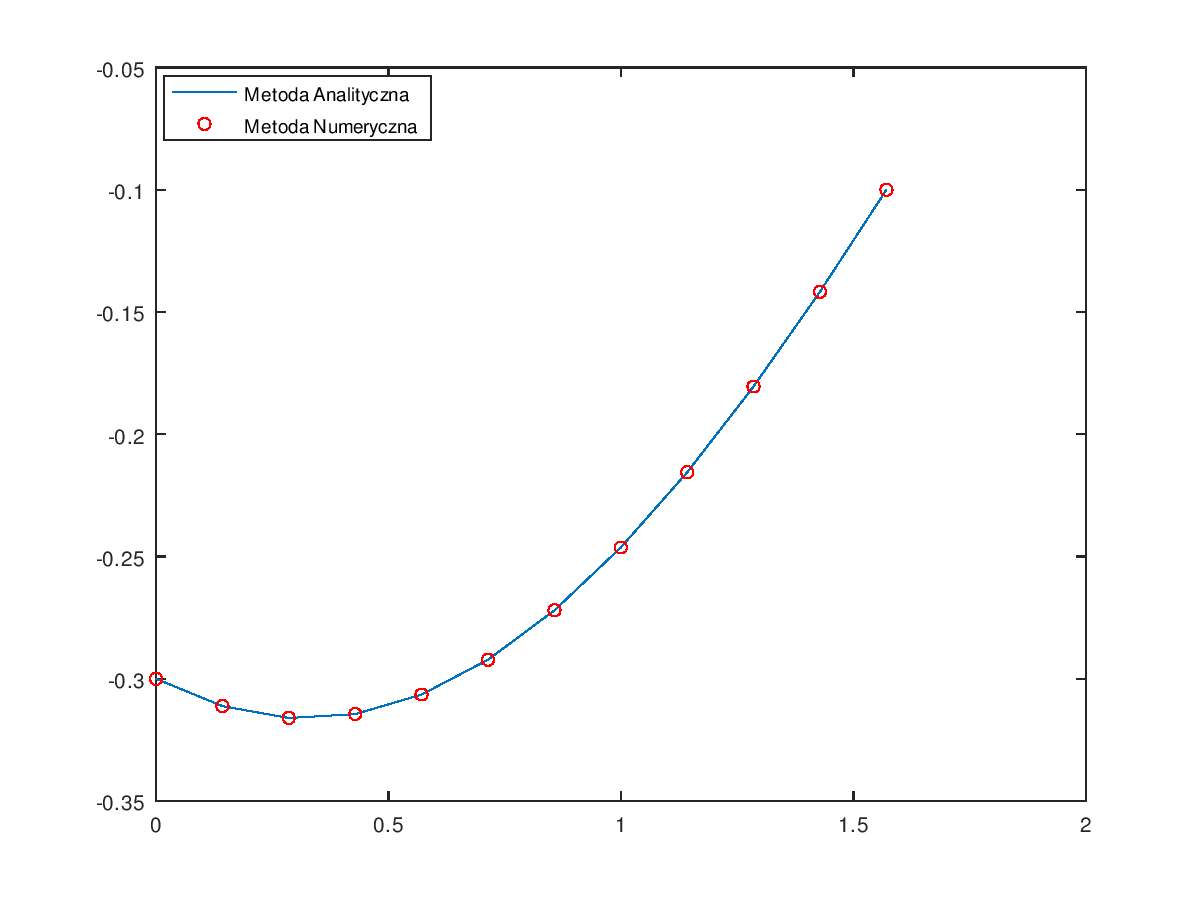
\includegraphics[width=0.8\textwidth]{Lab4/charts/zad2/zad2_n_10.png}
        \end{center}
        %\caption{Schemat logiczny w edytorze LAD oraz tabela symboli}
        %\label{fig:picture}
    \end{figure}
    \FloatBarrier
\end{samepage}

\begin{samepage}
    Dla 25 węzłów:
    \begin{figure}[!ht]
        \begin{center}
            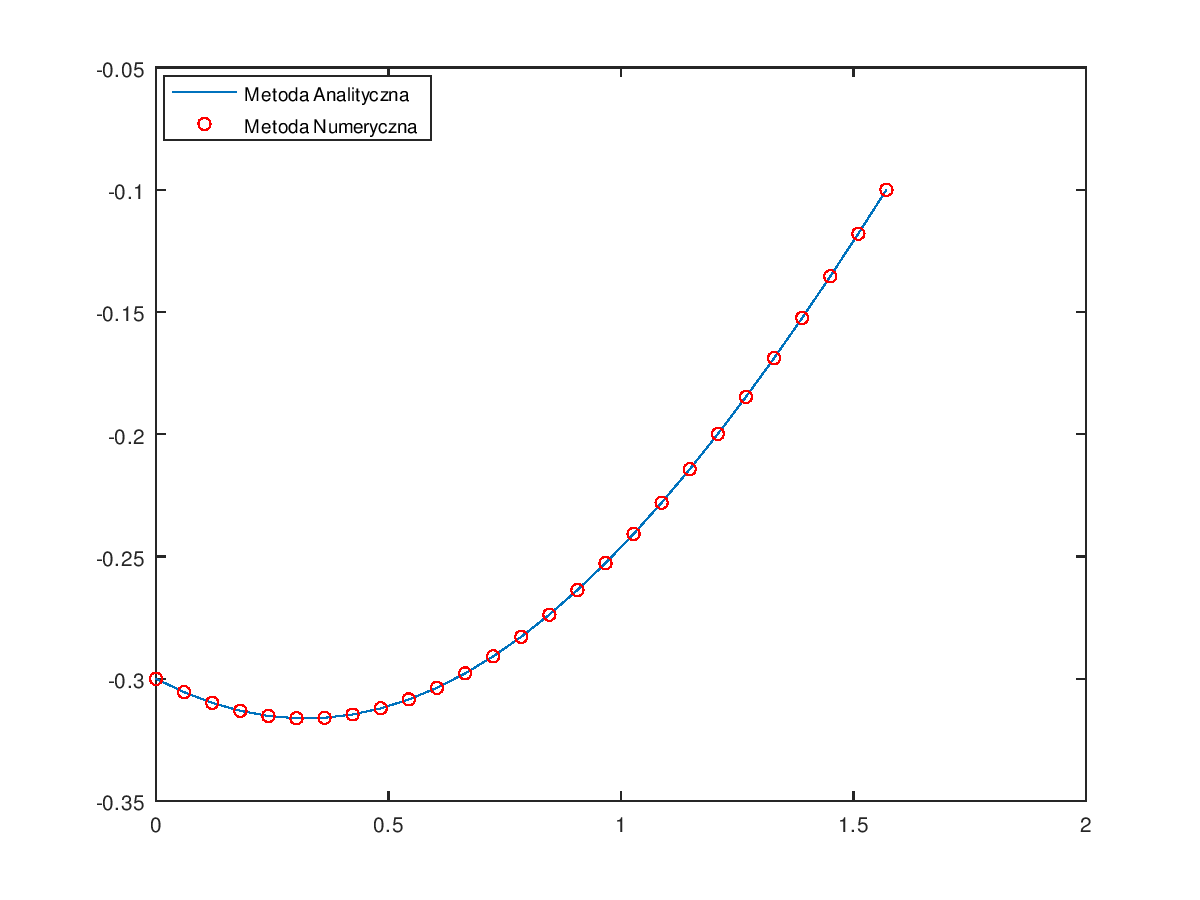
\includegraphics[width=0.8\textwidth]{Lab4/charts/zad2/zad2_n_25.png}
        \end{center}
        %\caption{Schemat logiczny w edytorze LAD oraz tabela symboli}
        %\label{fig:picture}
    \end{figure}
    \FloatBarrier
\end{samepage}

\newpage
\begin{samepage}
    
    Dla 100 węzłów:
    \begin{figure}[!ht]
        \begin{center}
            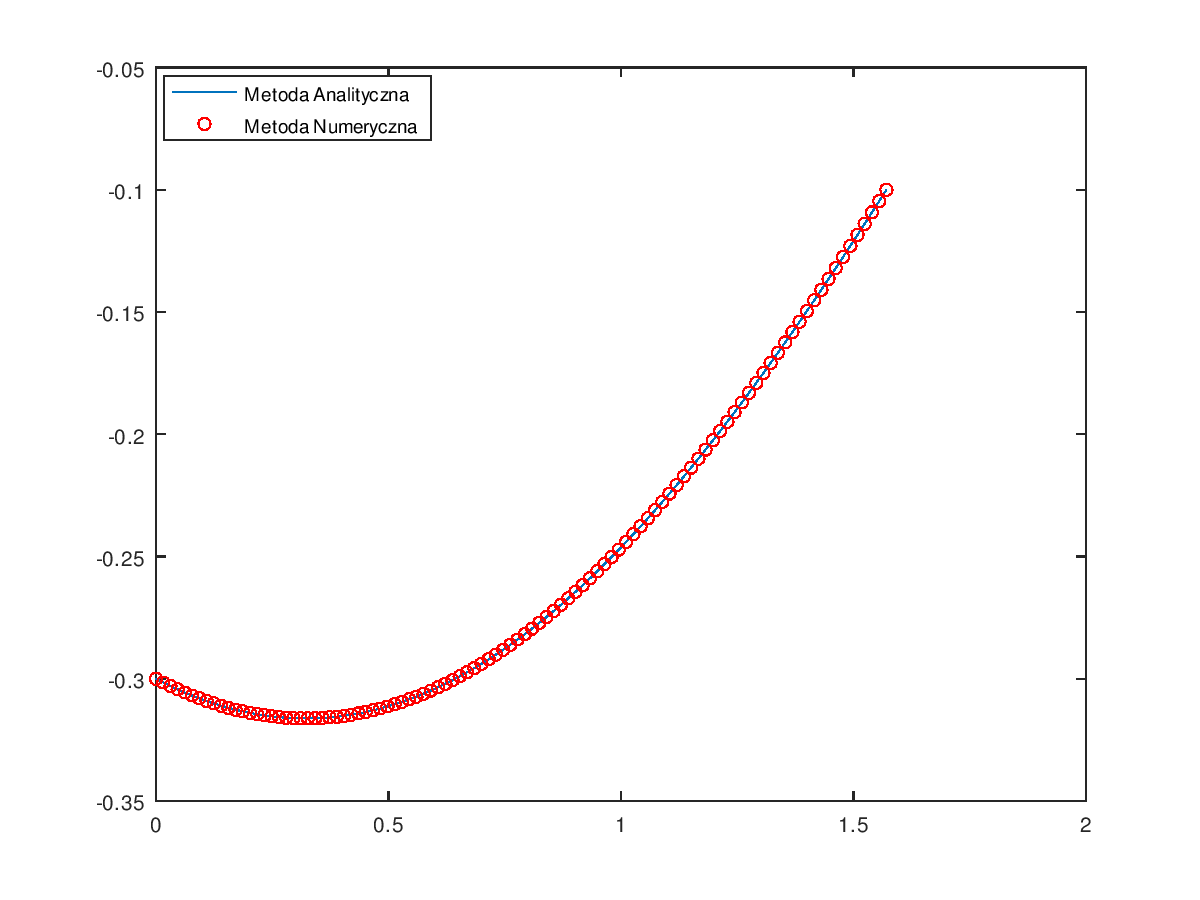
\includegraphics[width=0.8\textwidth]{Lab4/charts/zad2/zad2_n_100.png}
        \end{center}
        %\caption{Schemat logiczny w edytorze LAD oraz tabela symboli}
        %\label{fig:picture}
    \end{figure}
    \FloatBarrier
\end{samepage}


\begin{samepage}
    Dla 1000 węzłów:
    
    \begin{figure}[!ht]
        \begin{center}
            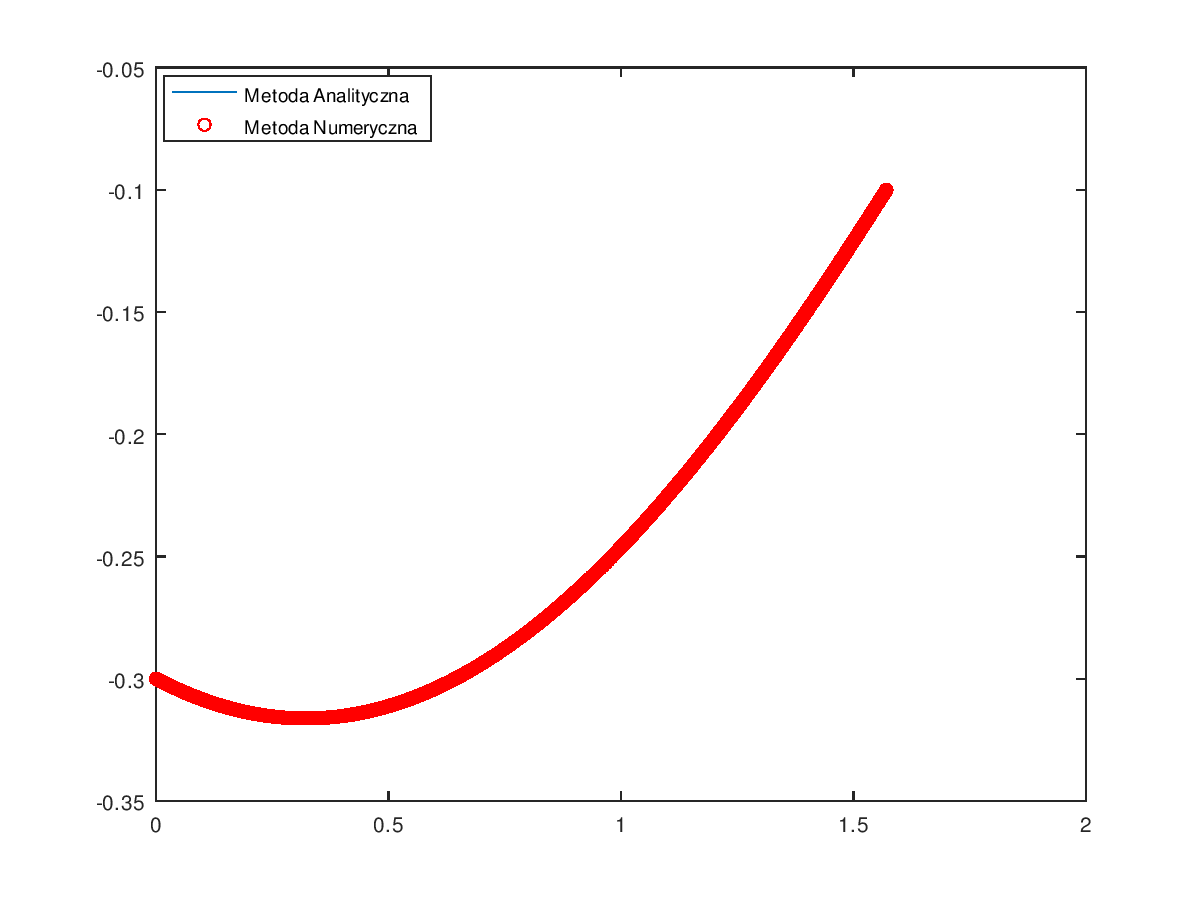
\includegraphics[width=0.8\textwidth]{Lab4/charts/zad2/zad2_n_1000.png}
        \end{center}
        %\caption{Schemat logiczny w edytorze LAD oraz tabela symboli}
        %\label{fig:picture}
    \end{figure}
    \FloatBarrier
\end{samepage}    

\newpage

\begin{samepage}
    Błąd metody w zależności od liczby węzłów:
    \begin{figure}[!ht]
        \begin{center}
            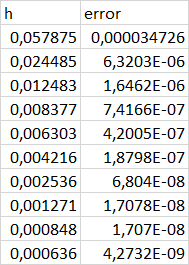
\includegraphics[width=0.8\textwidth]{Lab4/charts/zad2/error_dane.png}
        \end{center}
        %\caption{Schemat logiczny w edytorze LAD oraz tabela symboli}
        %\label{fig:picture}
    \end{figure}
    \FloatBarrier
\end{samepage} 

\begin{samepage}
    
    \begin{figure}[!ht]
        \begin{center}
            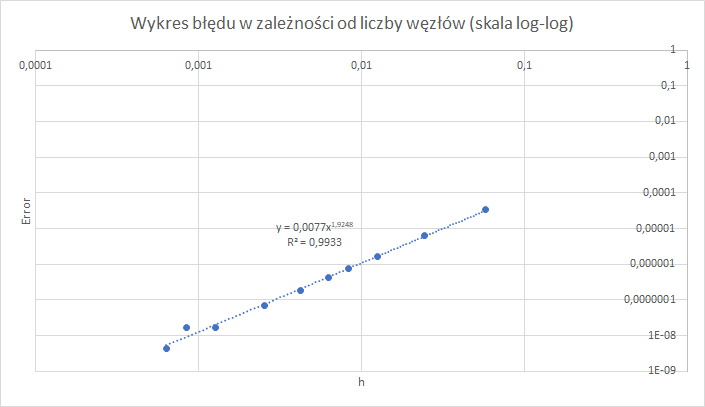
\includegraphics[width=0.8\textwidth]{Lab4/charts/zad2/error.png}
        \end{center}
        %\caption{Schemat logiczny w edytorze LAD oraz tabela symboli}
        %\label{fig:picture}
    \end{figure}
    \FloatBarrier
\end{samepage}   

\newpage
c)\\
\begin{samepage}
    Dla 10 węzłów:
    
    %{\centering
    
    %   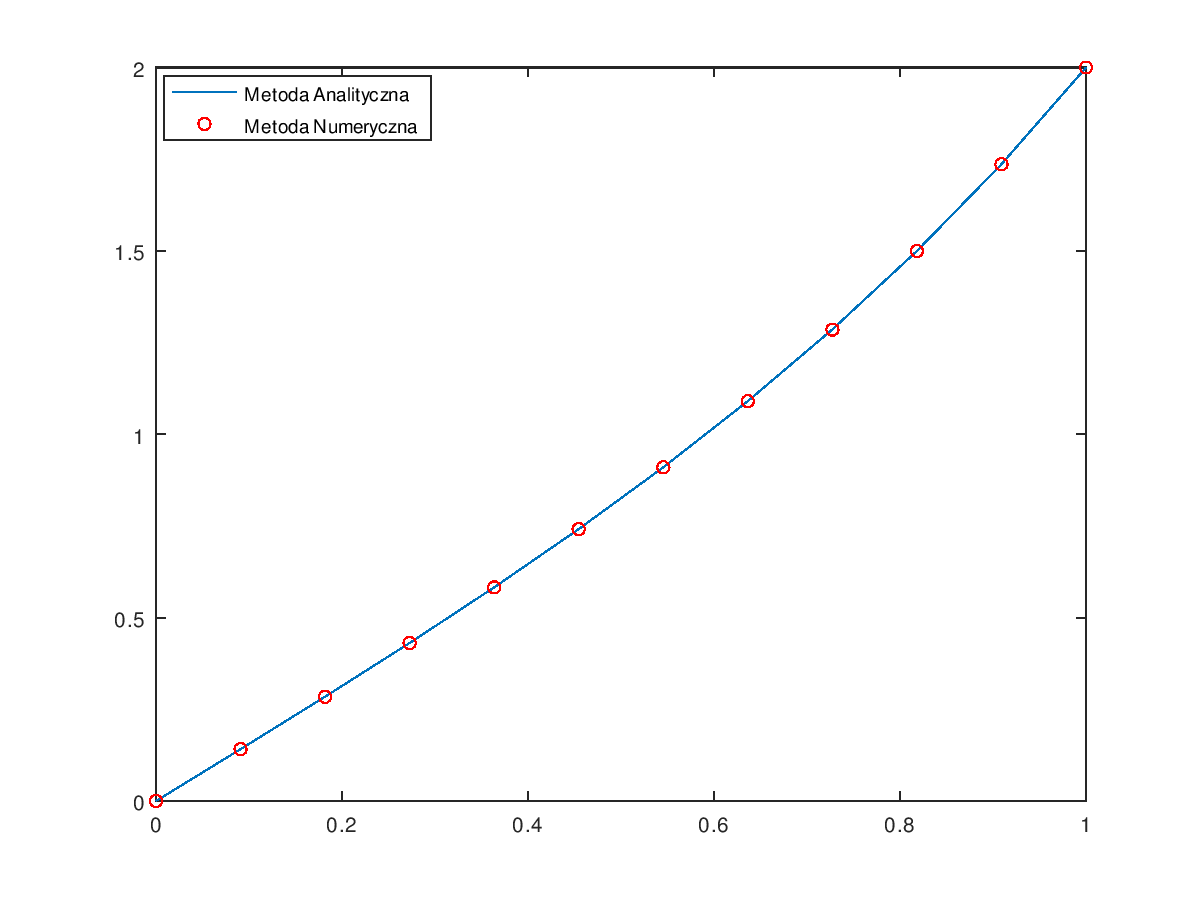
\includegraphics{Lab4/charts/zad1/zad1_n_10.png}
    
    %}
    \FloatBarrier
    \begin{figure}[!ht]
        \begin{center}
            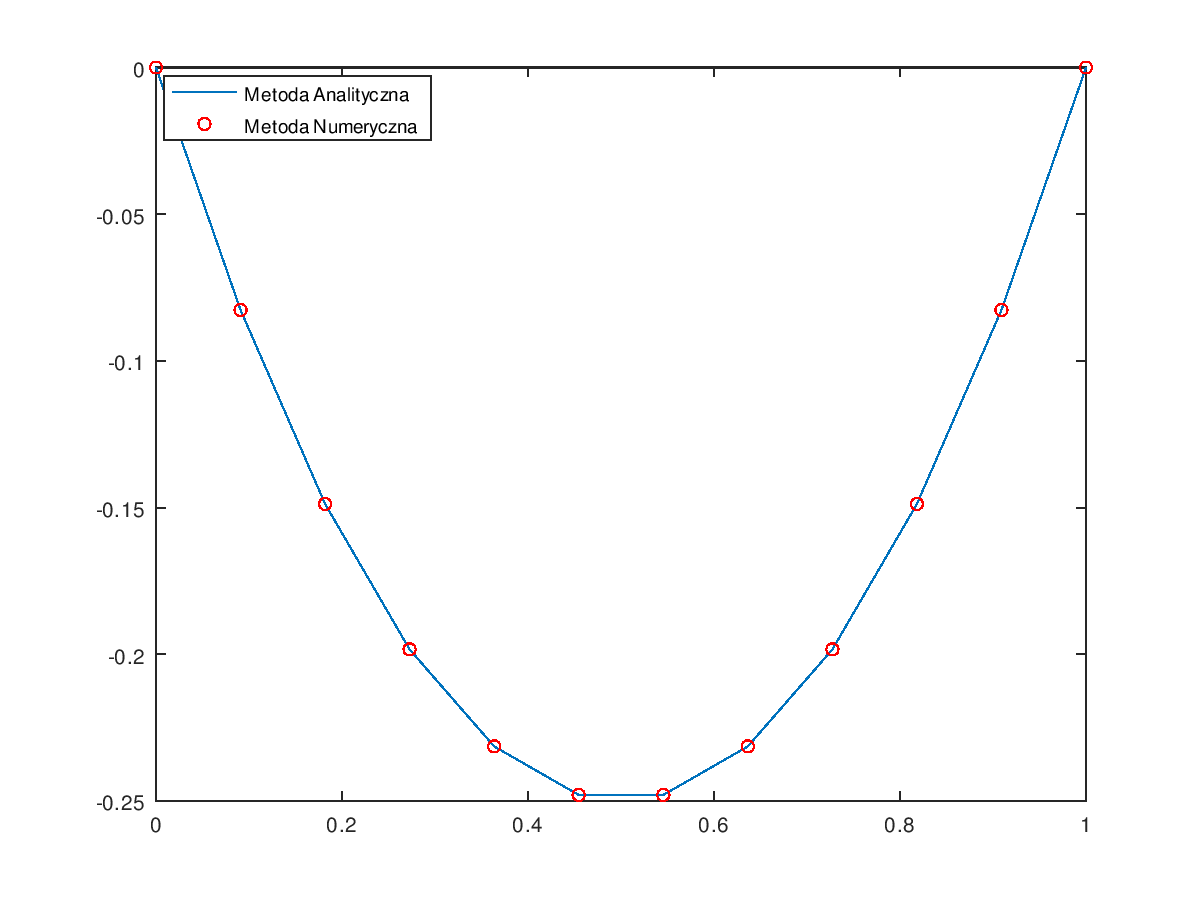
\includegraphics[width=0.8\textwidth]{Lab4/charts/zad3/zad3_n_10.png}
        \end{center}
        %\caption{Schemat logiczny w edytorze LAD oraz tabela symboli}
        %\label{fig:picture}
    \end{figure}
    \FloatBarrier
\end{samepage}

\begin{samepage}
    Dla 25 węzłów:
    \begin{figure}[!ht]
        \begin{center}
            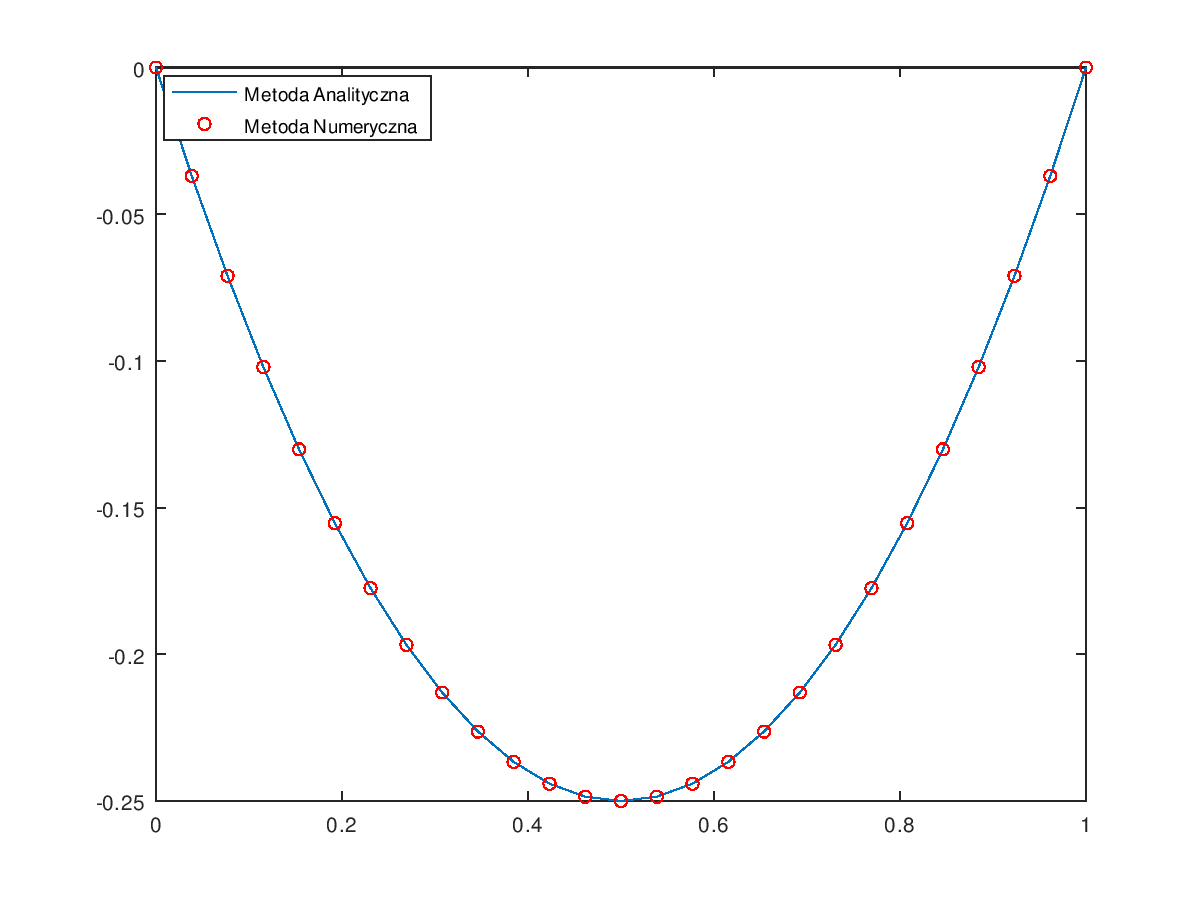
\includegraphics[width=0.8\textwidth]{Lab4/charts/zad3/zad3_n_25.png}
        \end{center}
        %\caption{Schemat logiczny w edytorze LAD oraz tabela symboli}
        %\label{fig:picture}
    \end{figure}
    \FloatBarrier
\end{samepage}

\newpage
\begin{samepage}
    
    Dla 100 węzłów:
    \begin{figure}[!ht]
        \begin{center}
            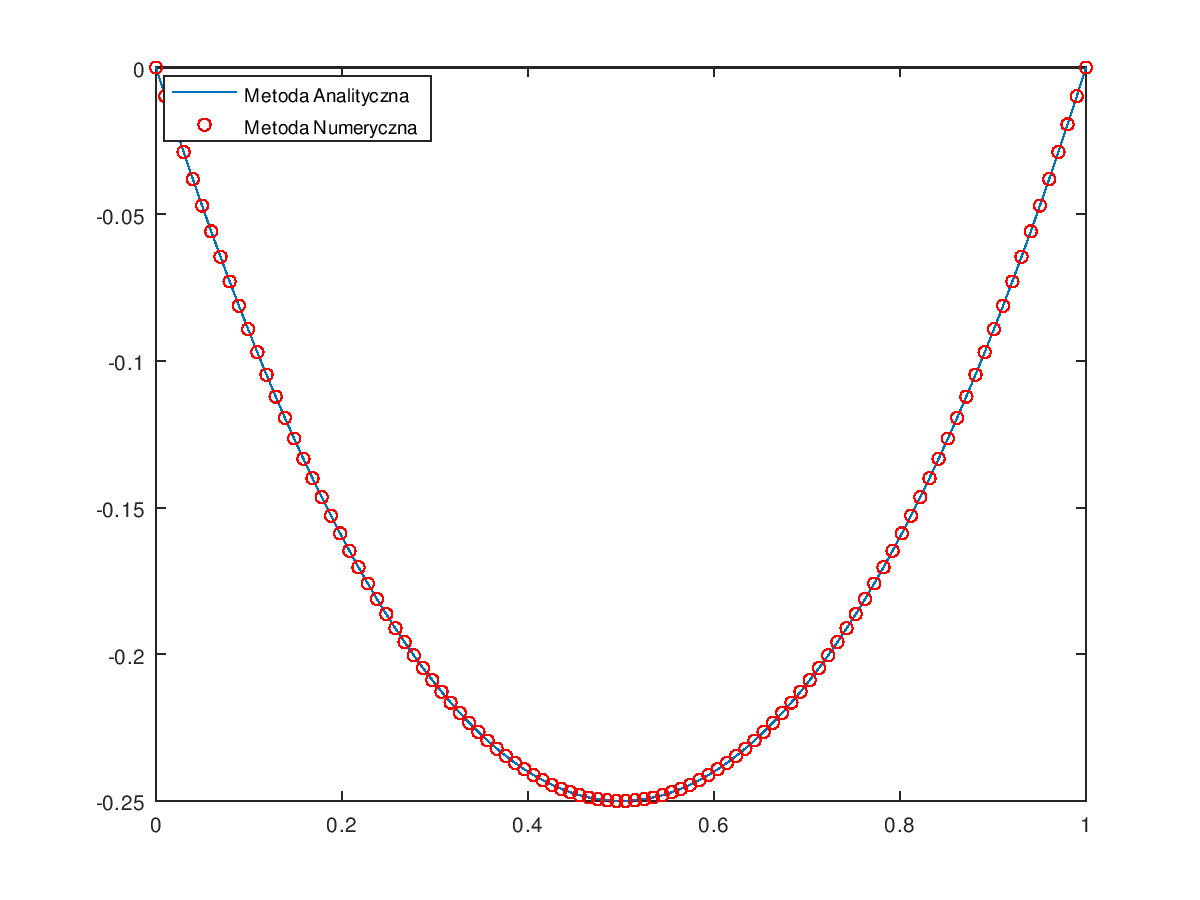
\includegraphics[width=0.8\textwidth]{Lab4/charts/zad3/zad3_n_100.png}
        \end{center}
        %\caption{Schemat logiczny w edytorze LAD oraz tabela symboli}
        %\label{fig:picture}
    \end{figure}
    \FloatBarrier
\end{samepage}


\begin{samepage}
    Dla 1000 węzłów:
    
    \begin{figure}[!ht]
        \begin{center}
            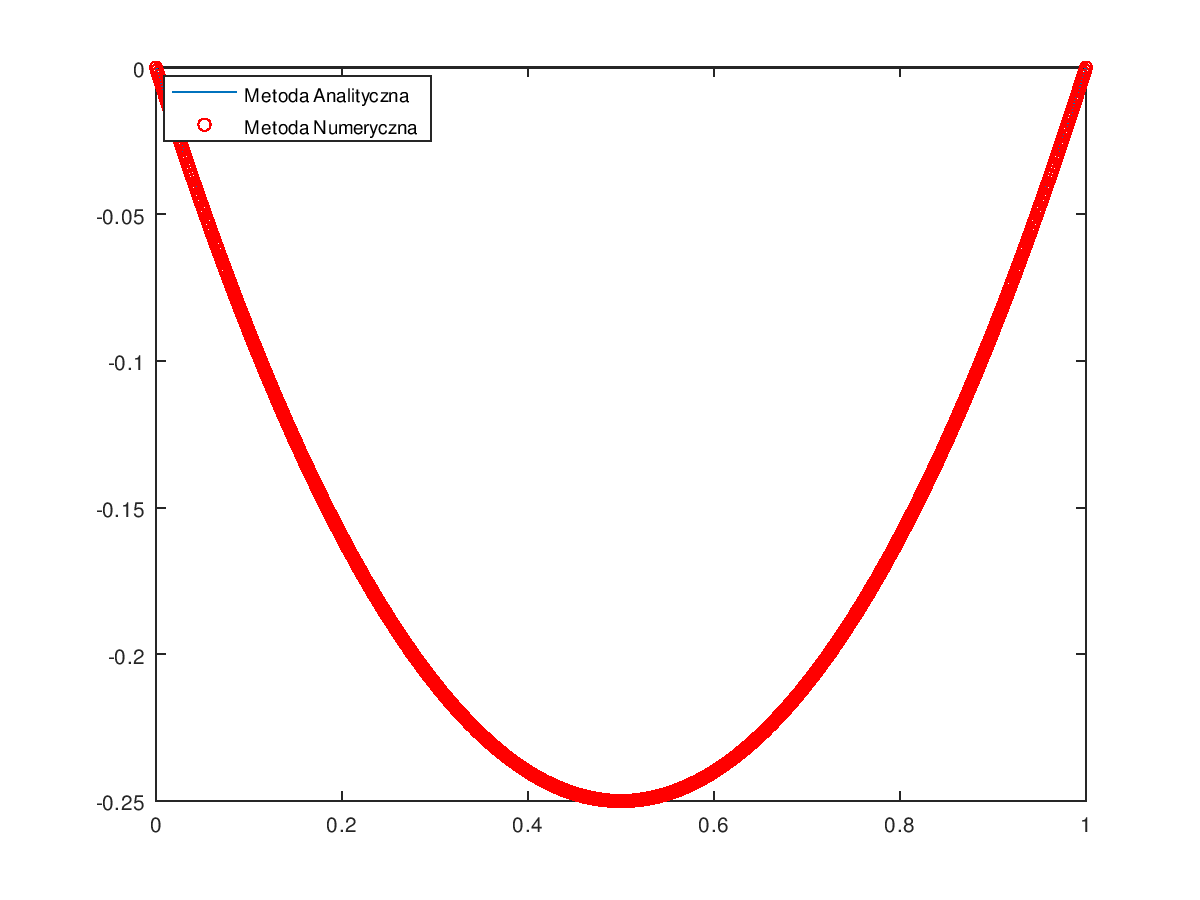
\includegraphics[width=0.8\textwidth]{Lab4/charts/zad3/zad3_n_1000.png}
        \end{center}
        %\caption{Schemat logiczny w edytorze LAD oraz tabela symboli}
        %\label{fig:picture}
    \end{figure}
    \FloatBarrier
\end{samepage}    

\newpage

\begin{samepage}
    Błąd metody w zależności od liczby węzłów:
    \begin{figure}[!ht]
        \begin{center}
            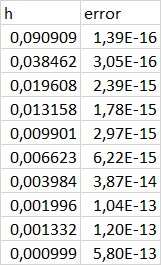
\includegraphics[width=0.8\textwidth]{Lab4/charts/zad3/error_dane.png}
        \end{center}
        %\caption{Schemat logiczny w edytorze LAD oraz tabela symboli}
        %\label{fig:picture}
    \end{figure}
    \FloatBarrier
\end{samepage} 

\begin{samepage}
    
    \begin{figure}[!ht]
        \begin{center}
            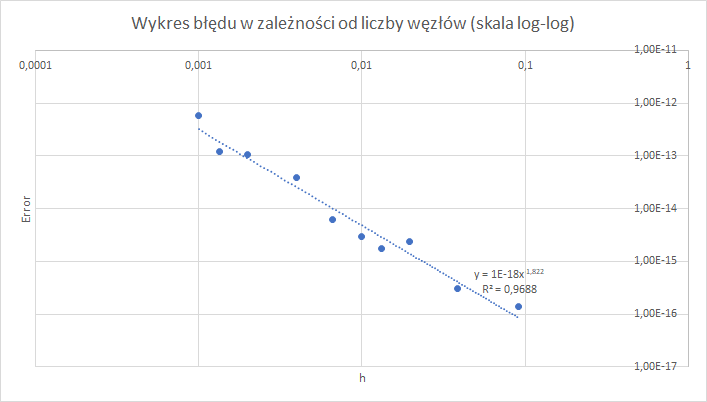
\includegraphics[width=0.8\textwidth]{Lab4/charts/zad3/error.png}
        \end{center}
        %\caption{Schemat logiczny w edytorze LAD oraz tabela symboli}
        %\label{fig:picture}
    \end{figure}
    \FloatBarrier
\end{samepage}   
    
    

\subsection{Warunki brzegowe typu Neumanna}
\textbf{Postać ogólna zagadnień brzegowych rzędu II z warunkami brzegowymi typu Neumanna:}

\[
\begin{cases}
\vspace{0.1cm} 
\hspace{0,1cm} a(x) u'' + b(x)u' + c(x)u =f(x) \\
\vspace{0.1cm}
\hspace{0,1cm}u'|_{x=a} = \widetilde{u}_{a} \\
\hspace{0,1cm}u|_{x=b} = u_{b}
\end{cases}
\]
, gdzie:
$x\in[a,b]$
\\

\subsection{Cel ćwiczenia}
Kolejnym zadaniem było stworzenie algorytmów rozwiązujących zagadnienia brzegowe II rzędu z warunkami brzegowymi typu Neumanna.
\\\\
a) Pierwszego podejście polegało na wykorzystaniu schematu jednostronnego w celu aproksymacji pochodnej rzędu I występującej w warunku brzegowym typu Neumanna
\newpage
b) Drugie podejście polegało na dołączeniu dodatkowego węzła o indeksie (-1), który w rzeczywistości nie występuje w układzie równań
\\\\
c) Trzecie podejście polegało na wykorzystaniu jednostronnych schematów w węźle brzegowym
%\newpage

Do rozwiązania zostało podane następujące zagadnienie:
\[
\begin{cases}
\vspace{0.1cm} 
\hspace{0,1cm}u''-xu' + u=e^x(-x^2+x+2) \\
\vspace{0.1cm}
\hspace{0,1cm}u|_{x=0}=0 \\
\hspace{0,1cm}u'|_{x=1}=2e
\end{cases}
\]
, gdzie:

$x\in [0,1]$
\\
Rozwiązanie analityczne: $\widetilde{u}(x) = (x+1)e^x$

\subsection{Algorytm}

\begin{samepage}
a)
\begin{Shaded}
\begin{Highlighting}[]
\FunctionTok{clear}\NormalTok{, }\FunctionTok{clc}\NormalTok{;}
\CommentTok{# Dane wejściowe}
\NormalTok{f = @(x) }\FunctionTok{exp}\NormalTok{(x) .* (-x .^}\FloatTok{2} \NormalTok{+ x + }\FloatTok{2}\NormalTok{);}
\NormalTok{g = @(x) x .* }\FunctionTok{exp}\NormalTok{(x);}
\NormalTok{a = }\FloatTok{0}\NormalTok{;}
\NormalTok{b = }\FloatTok{1}\NormalTok{;}
\NormalTok{ax = @(x) }\FloatTok{1}\NormalTok{;}
\NormalTok{bx = @(x) -x;}
\NormalTok{cx = @(x) }\FloatTok{1}\NormalTok{;}
\NormalTok{ua = }\FloatTok{0}\NormalTok{;}
\NormalTok{ubf = }\FloatTok{2} \NormalTok{* }\FunctionTok{exp}\NormalTok{(}\FloatTok{1}\NormalTok{);}
\NormalTok{c = b-a;}
\NormalTok{n = }\FloatTok{10}\NormalTok{;}
\NormalTok{h = c/(n+}\FloatTok{1}\NormalTok{);}
\NormalTok{x = }\FunctionTok{linspace}\NormalTok{((a+h),(b-h),n);}
\CommentTok{# Obliczenia}
\NormalTok{a1 = [(-}\FloatTok{2} \NormalTok{* ax(x) + cx(x) * h^}\FloatTok{2}\NormalTok{).* }\FunctionTok{diag}\NormalTok{(}\FunctionTok{eye}\NormalTok{(n)); }\FloatTok{1}\NormalTok{];}
\NormalTok{A1 = }\FunctionTok{diag}\NormalTok{(a1);}
\NormalTok{a2 = (ax(x) +}\FloatTok{1}\NormalTok{/}\FloatTok{2} \NormalTok{* bx(x) * h)' .* }\FunctionTok{diag}\NormalTok{(}\FunctionTok{eye}\NormalTok{(n));}
\NormalTok{A2 = }\FunctionTok{diag}\NormalTok{(a2, }\FloatTok{1}\NormalTok{);}
\NormalTok{a3 = [(ax(x(}\FloatTok{2}\NormalTok{:n)) -}\FloatTok{1}\NormalTok{/}\FloatTok{2} \NormalTok{* bx(x(}\FloatTok{2}\NormalTok{:n)) * h)' .* }\FunctionTok{diag}\NormalTok{(}\FunctionTok{eye}\NormalTok{(n-}\FloatTok{1}\NormalTok{)); -}\FloatTok{1}\NormalTok{];}
\NormalTok{A3 = }\FunctionTok{diag}\NormalTok{(a3, -}\FloatTok{1}\NormalTok{);}
\NormalTok{A = A1  + A2 + A3;}
\NormalTok{F = h^}\FloatTok{2} \NormalTok{* f(x);}
\NormalTok{F(}\FloatTok{1}\NormalTok{) = F(}\FloatTok{1}\NormalTok{) - ua;}
\NormalTok{F = [F h*ubf];}
\NormalTok{U = linsolve(A,F');}
\NormalTok{U = [ua U'];}
\NormalTok{X = [a x b];}
\CommentTok{# Wykres}
\FunctionTok{plot}\NormalTok{(X, U, X, g(X), }\StringTok{'ro'}\NormalTok{);}
\CommentTok{# Błąd}
\NormalTok{E = }\FunctionTok{max}\NormalTok{(}\FunctionTok{abs}\NormalTok{(g(X) - U));}
\end{Highlighting}
\end{Shaded}

\end{samepage}
\newpage
\begin{samepage}
b)
\begin{Shaded}
\begin{Highlighting}[]
\FunctionTok{clear}\NormalTok{, }\FunctionTok{clc}\NormalTok{;}
\CommentTok{# Dane wejściowe}
\NormalTok{f = @(x) }\FunctionTok{exp}\NormalTok{(x) .* (-x .^}\FloatTok{2} \NormalTok{+ x + }\FloatTok{2}\NormalTok{);}
\NormalTok{g = @(x) x .* }\FunctionTok{exp}\NormalTok{(x);}
\NormalTok{a = }\FloatTok{0}\NormalTok{;}
\NormalTok{b = }\FloatTok{1}\NormalTok{;}
\NormalTok{ax = @(x) }\FloatTok{1}\NormalTok{;}
\NormalTok{bx = @(x) -x;}
\NormalTok{cx = @(x) }\FloatTok{1}\NormalTok{;}
\NormalTok{ua = }\FloatTok{0}\NormalTok{;}
\NormalTok{ubf = }\FloatTok{2} \NormalTok{* }\FunctionTok{exp}\NormalTok{(}\FloatTok{1}\NormalTok{);}
\NormalTok{c = b-a;}
\NormalTok{n = }\FloatTok{10}\NormalTok{;}
\NormalTok{h = c/(n+}\FloatTok{1}\NormalTok{);}
\NormalTok{x = }\FunctionTok{linspace}\NormalTok{((a+h),(b-h),n);}
\CommentTok{# Obliczenia}
\NormalTok{a1 = [(-}\FloatTok{2} \NormalTok{* ax(x) + cx(x) * h^}\FloatTok{2}\NormalTok{).* }\FunctionTok{diag}\NormalTok{(}\FunctionTok{eye}\NormalTok{(n)); -}\FloatTok{1}\NormalTok{];}
\NormalTok{A1 = }\FunctionTok{diag}\NormalTok{(a1);}
\NormalTok{a2 = (ax(x) +}\FloatTok{1}\NormalTok{/}\FloatTok{2} \NormalTok{* bx(x) * h)' .* }\FunctionTok{diag}\NormalTok{(}\FunctionTok{eye}\NormalTok{(n));}
\NormalTok{A2 = }\FunctionTok{diag}\NormalTok{(a2, }\FloatTok{1}\NormalTok{);}
\NormalTok{a3 = [(ax(x(}\FloatTok{2}\NormalTok{:n)) -}\FloatTok{1}\NormalTok{/}\FloatTok{2} \NormalTok{* bx(x(}\FloatTok{2}\NormalTok{:n)) * h)' .* }\FunctionTok{diag}\NormalTok{(}\FunctionTok{eye}\NormalTok{(n-}\FloatTok{1}\NormalTok{)); }\FloatTok{1}\NormalTok{];}
\NormalTok{A3 = }\FunctionTok{diag}\NormalTok{(a3, -}\FloatTok{1}\NormalTok{);}
\NormalTok{A = A1  + A2 + A3;}
\NormalTok{F = h^}\FloatTok{2} \NormalTok{* f(x);}
\NormalTok{F(}\FloatTok{1}\NormalTok{) = F(}\FloatTok{1}\NormalTok{) - ua;}
\NormalTok{F = [F }\FloatTok{1}\NormalTok{/}\FloatTok{2} \NormalTok{* h^}\FloatTok{2}\NormalTok{*f(b) - h * ubf];}
\NormalTok{U = linsolve(A,F');}
\NormalTok{U = [ua U'];}
\NormalTok{X = [a x b];}
\CommentTok{# Wykres}
\FunctionTok{plot}\NormalTok{(X, U, X, g(X), }\StringTok{'ro'}\NormalTok{);}
\CommentTok{# Błąd}
\NormalTok{E = }\FunctionTok{max}\NormalTok{(}\FunctionTok{abs}\NormalTok{(g(X) - U));}
\end{Highlighting}
\end{Shaded}

\end{samepage}
\newpage
\begin{samepage}
c)
\begin{Shaded}
\begin{Highlighting}[]
\FunctionTok{clear}\NormalTok{, }\FunctionTok{clc}\NormalTok{;}
\CommentTok{# Dane wejściowe}
\NormalTok{f = @(x) }\FunctionTok{exp}\NormalTok{(x) .* (-x .^}\FloatTok{2} \NormalTok{+ x + }\FloatTok{2}\NormalTok{);}
\NormalTok{g = @(x) (x) .* }\FunctionTok{exp}\NormalTok{(x);}
\NormalTok{a = }\FloatTok{0}\NormalTok{;}
\NormalTok{b = }\FloatTok{1}\NormalTok{;}
\NormalTok{ax = @(x) }\FloatTok{1}\NormalTok{;}
\NormalTok{bx = @(x) -x;}
\NormalTok{cx = @(x) }\FloatTok{1}\NormalTok{;}
\NormalTok{ua = }\FloatTok{0}\NormalTok{;}
\NormalTok{ubf = }\FloatTok{2} \NormalTok{* }\FunctionTok{exp}\NormalTok{(}\FloatTok{1}\NormalTok{);}
\NormalTok{c = b-a;}
\NormalTok{n = }\FloatTok{10}\NormalTok{;}
\NormalTok{h = c/(n+}\FloatTok{1}\NormalTok{);}
\NormalTok{x = }\FunctionTok{linspace}\NormalTok{((a+h),(b-h),n);}
\CommentTok{# Obliczenia}
\NormalTok{a1 = [(-}\FloatTok{2} \NormalTok{* ax(x) + cx(x) * h^}\FloatTok{2}\NormalTok{).* }\FunctionTok{diag}\NormalTok{(}\FunctionTok{eye}\NormalTok{(n)); }\FloatTok{3}\NormalTok{];}
\NormalTok{A1 = }\FunctionTok{diag}\NormalTok{(a1);}
\NormalTok{a2 = (ax(x) +}\FloatTok{1}\NormalTok{/}\FloatTok{2} \NormalTok{* bx(x) * h)' .* }\FunctionTok{diag}\NormalTok{(}\FunctionTok{eye}\NormalTok{(n));}
\NormalTok{A2 = }\FunctionTok{diag}\NormalTok{(a2, }\FloatTok{1}\NormalTok{);}
\NormalTok{a3 = [(ax(x(}\FloatTok{2}\NormalTok{:n)) -}\FloatTok{1}\NormalTok{/}\FloatTok{2} \NormalTok{* bx(x(}\FloatTok{2}\NormalTok{:n)) * h)' .* }\FunctionTok{diag}\NormalTok{(}\FunctionTok{eye}\NormalTok{(n-}\FloatTok{1}\NormalTok{)); -}\FloatTok{4}\NormalTok{];}
\NormalTok{A3 = }\FunctionTok{diag}\NormalTok{(a3, -}\FloatTok{1}\NormalTok{);}
\NormalTok{a4 = [}\FunctionTok{zeros}\NormalTok{(n-}\FloatTok{2}\NormalTok{,}\FloatTok{1}\NormalTok{); }\FloatTok{1}\NormalTok{];}
\NormalTok{A4 = }\FunctionTok{diag}\NormalTok{(a4, -}\FloatTok{2}\NormalTok{);}
\NormalTok{A = A1 + A2 + A3 + A4;}
\NormalTok{F = h^}\FloatTok{2} \NormalTok{* f(x);}
\NormalTok{F(}\FloatTok{1}\NormalTok{) = F(}\FloatTok{1}\NormalTok{) - ua;}
\NormalTok{F = [F }\FloatTok{2}\NormalTok{*h*ubf];}
\NormalTok{U = linsolve(A,F');}
\NormalTok{U = [ua U'];}
\NormalTok{X = [a x b];}
\CommentTok{# Wykres}
\FunctionTok{plot}\NormalTok{(X, U, X, g(X), }\StringTok{'ro'}\NormalTok{);}
\CommentTok{# Błąd}
\NormalTok{E = }\FunctionTok{max}\NormalTok{(}\FunctionTok{abs}\NormalTok{(g(X) - U));}
\end{Highlighting}
\end{Shaded}
\end{samepage}

\newpage

\subsection{Wykresy}

a)

\begin{samepage}
	Dla 10 węzłów:
	
	\FloatBarrier
	\begin{figure}[!ht]
		\begin{center}
			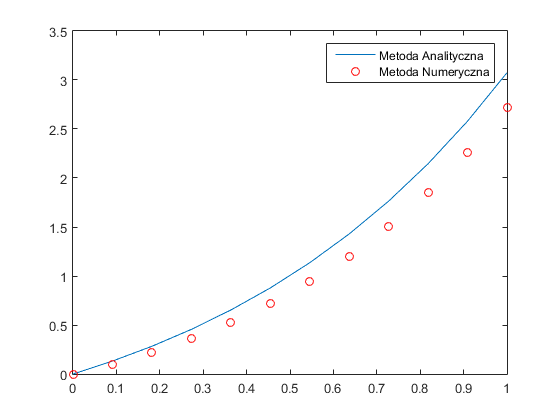
\includegraphics[width=0.8\textwidth]{Lab4/charts/zad4/a/10.png}
		\end{center}
	\end{figure}
	\FloatBarrier
\end{samepage}

\begin{samepage}
	Dla 25 węzłów:
	
	\FloatBarrier
	\begin{figure}[!ht]
		\begin{center}
			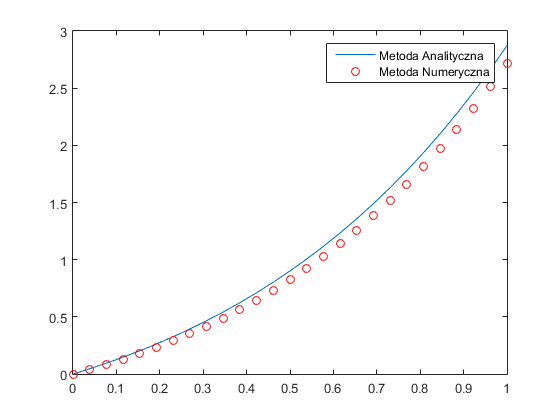
\includegraphics[width=0.8\textwidth]{Lab4/charts/zad4/a/25.png}
		\end{center}
	\end{figure}
	\FloatBarrier
\end{samepage}

\newpage

\begin{samepage}
	Dla 100 węzłów:
	
	\FloatBarrier
	\begin{figure}[!ht]
		\begin{center}
			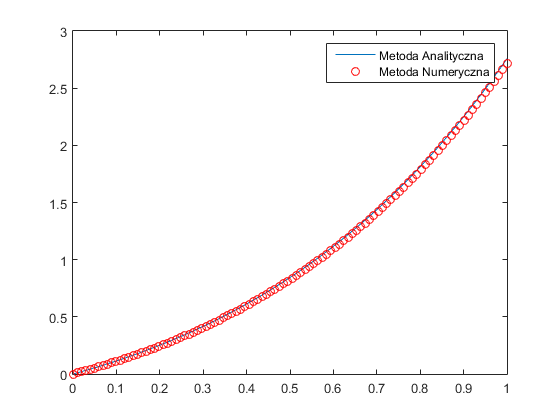
\includegraphics[width=0.8\textwidth]{Lab4/charts/zad4/a/100.png}
		\end{center}
	\end{figure}
	\FloatBarrier
\end{samepage}

\begin{samepage}
	Dla 1000 węzłów:
	
	\FloatBarrier
	\begin{figure}[!ht]
		\begin{center}
			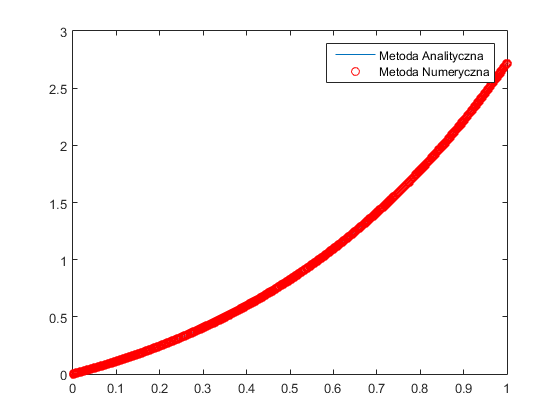
\includegraphics[width=0.8\textwidth]{Lab4/charts/zad4/a/1000.png}
		\end{center}
	\end{figure}
	\FloatBarrier
\end{samepage}

\newpage

Błąd metody w zależności od liczby węzłów:

\begin{samepage}
	\FloatBarrier
	\begin{figure}[!ht]
		\begin{center}
			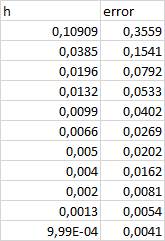
\includegraphics[width=0.8\textwidth]{Lab4/charts/zad4/a/error_dane.png}
		\end{center}
	\end{figure}
	\FloatBarrier
\end{samepage}

\begin{samepage}

	\FloatBarrier
	\begin{figure}[!ht]
		\begin{center}
			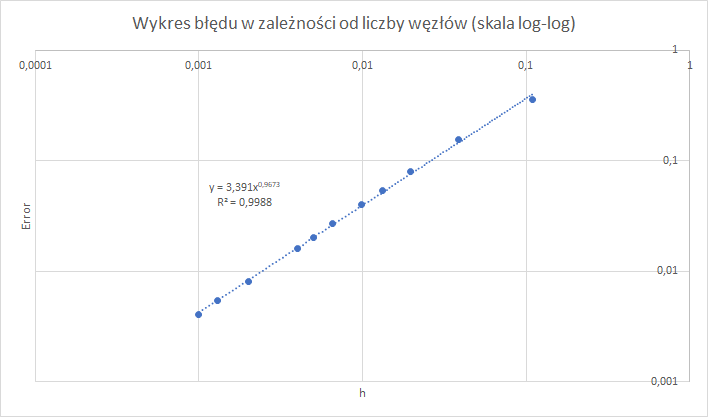
\includegraphics[width=0.8\textwidth]{Lab4/charts/zad4/a/error.png}
		\end{center}
	\end{figure}
	\FloatBarrier
\end{samepage}

\newpage

b)

\begin{samepage}
	Dla 10 węzłów:
	
	\FloatBarrier
	\begin{figure}[!ht]
		\begin{center}
			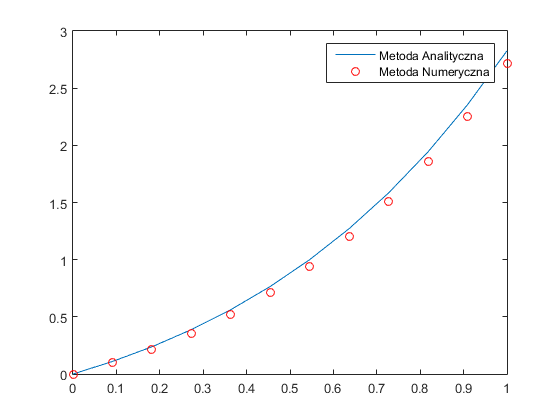
\includegraphics[width=0.8\textwidth]{Lab4/charts/zad4/b/10.png}
		\end{center}
	\end{figure}
	\FloatBarrier
\end{samepage}

\begin{samepage}
	Dla 25 węzłów:
	
	\FloatBarrier
	\begin{figure}[!ht]
		\begin{center}
			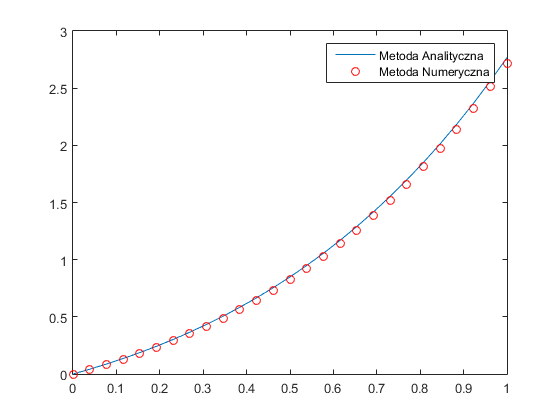
\includegraphics[width=0.8\textwidth]{Lab4/charts/zad4/b/25.png}
		\end{center}
	\end{figure}
	\FloatBarrier
\end{samepage}

\newpage

\begin{samepage}
	Dla 100 węzłów:
	
	\FloatBarrier
	\begin{figure}[!ht]
		\begin{center}
			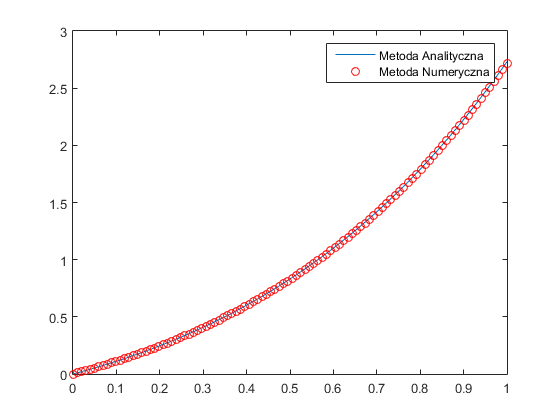
\includegraphics[width=0.8\textwidth]{Lab4/charts/zad4/b/100.png}
		\end{center}
	\end{figure}
	\FloatBarrier
\end{samepage}

\begin{samepage}
	Dla 1000 węzłów:
	
	\FloatBarrier
	\begin{figure}[!ht]
		\begin{center}
			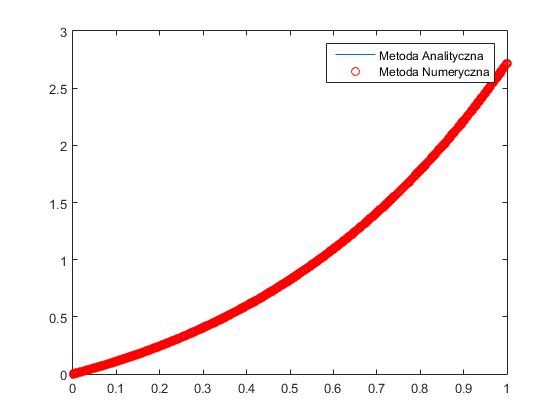
\includegraphics[width=0.8\textwidth]{Lab4/charts/zad4/b/1000.png}
		\end{center}
	\end{figure}
	\FloatBarrier
\end{samepage}

\newpage

Błąd metody w zależności od liczby węzłów:

\begin{samepage}
	\FloatBarrier
	\begin{figure}[!ht]
		\begin{center}
			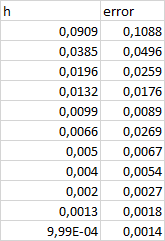
\includegraphics[width=0.8\textwidth]{Lab4/charts/zad4/b/error_dane.png}
		\end{center}
	\end{figure}
	\FloatBarrier
\end{samepage}

\begin{samepage}
	
	\FloatBarrier
	\begin{figure}[!ht]
		\begin{center}
			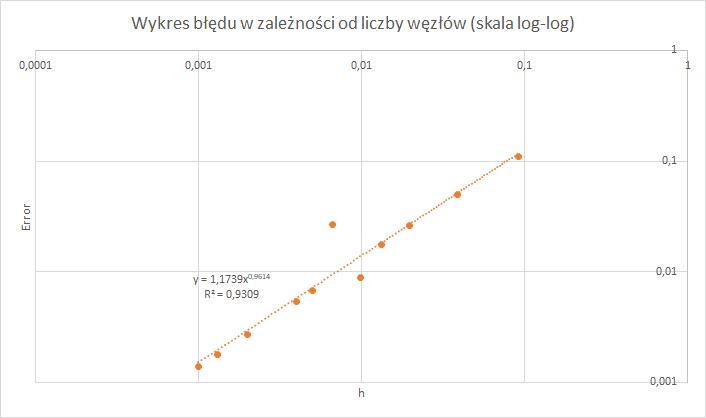
\includegraphics[width=0.8\textwidth]{Lab4/charts/zad4/b/error.png}
		\end{center}
	\end{figure}
	\FloatBarrier
\end{samepage}

\newpage

c)

\begin{samepage}
	Dla 10 węzłów:
	
	\FloatBarrier
	\begin{figure}[!ht]
		\begin{center}
			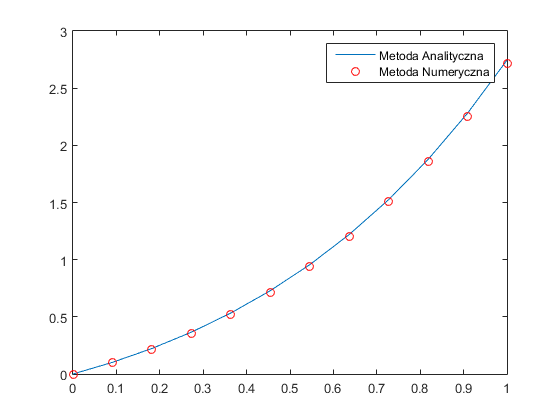
\includegraphics[width=0.8\textwidth]{Lab4/charts/zad4/c/10.png}
		\end{center}
	\end{figure}
	\FloatBarrier
\end{samepage}

\begin{samepage}
	Dla 25 węzłów:
	
	\FloatBarrier
	\begin{figure}[!ht]
		\begin{center}
			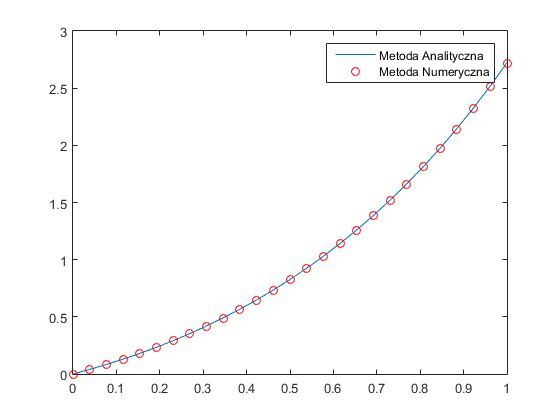
\includegraphics[width=0.8\textwidth]{Lab4/charts/zad4/c/25.png}
		\end{center}
	\end{figure}
	\FloatBarrier
\end{samepage}

\newpage

\begin{samepage}
	Dla 100 węzłów:
	
	\FloatBarrier
	\begin{figure}[!ht]
		\begin{center}
			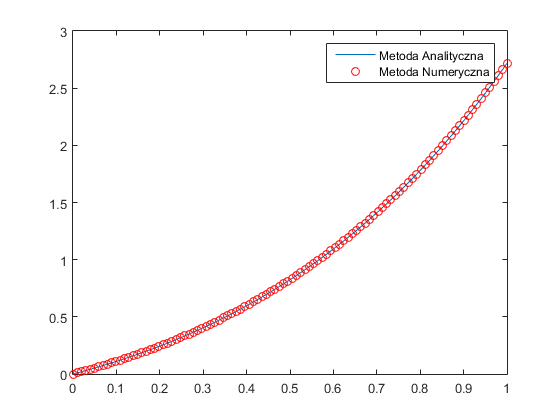
\includegraphics[width=0.8\textwidth]{Lab4/charts/zad4/c/100.png}
		\end{center}
	\end{figure}
	\FloatBarrier
\end{samepage}

\begin{samepage}
	Dla 1000 węzłów:
	
	\FloatBarrier
	\begin{figure}[!ht]
		\begin{center}
			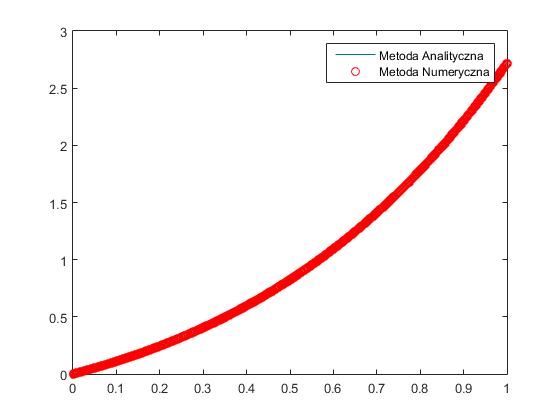
\includegraphics[width=0.8\textwidth]{Lab4/charts/zad4/c/1000.png}
		\end{center}
	\end{figure}
	\FloatBarrier
\end{samepage}

\newpage

Błąd metody w zależności od liczby węzłów:

\begin{samepage}
	\FloatBarrier
	\begin{figure}[!ht]
		\begin{center}
			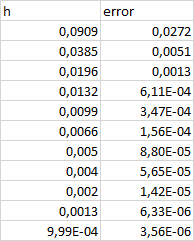
\includegraphics[width=0.8\textwidth]{Lab4/charts/zad4/c/error_dane.png}
		\end{center}
	\end{figure}
	\FloatBarrier
\end{samepage}

\begin{samepage}
	
	\FloatBarrier
	\begin{figure}[!ht]
		\begin{center}
			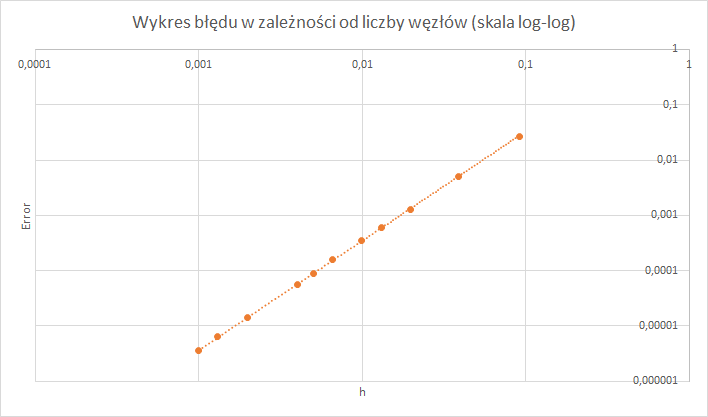
\includegraphics[width=0.8\textwidth]{Lab4/charts/zad4/c/error.png}
		\end{center}
	\end{figure}
	\FloatBarrier
\end{samepage}






